\documentclass[a4paper,11pt]{report}

\usepackage{amsmath}
\usepackage{graphicx}

\begin{document}

\section*{Single phase flow: governing equation}

We write Navier-Stokes equations as

\begin{equation}
    \label{eqn:NavierStokes}
    \begin{aligned}
        &\nabla \cdot \vec{u} = 0 \\
        &\rho\left(\partial_t \vec{u} + \vec{u} \cdot \nabla \vec{u}\right) = -\nabla p + \mu \nabla^2 \vec{u} + \rho \vec{f}
    \end{aligned}
\end{equation}
%
with $\vec{u} = \vec{u}\left(\vec{x},t\right)$ the velocity field, $p = p(\vec{x},t)$ the pressure field, $\rho$ the density,
$\mu$ the viscosity and $\vec{f}$ external volume forces.

\section*{Time discretization: predictor-corrector}

The unknowns in \eqref{eqn:NavierStokes} are $\vec{u}$ and $p$. A 2nd-order central scheme time discretization of equation \eqref{eqn:NavierStokes}, which contains both variables at new timestep, correspond to
\begin{equation}
    \label{eqn:2ndOrderTime}
    \begin{aligned}
        &\frac{\vec{u}^{\, n+1} - \vec{u}^{\, n}}{\Delta t} = \\
        &= \frac{1}{\rho}\left[-\nabla p^{n+1} - \vec{u}^{\, n+1/2} \cdot \nabla \vec{u}^{\, n+1/2} + \mu \nabla^2 \vec{u}^{\, n+1/2} + \rho \vec{f}^{\, n+1/2}\right]
    \end{aligned}
\end{equation}
with $\vec{u}^{\, n} = \vec{u}\left(\vec{x},n\Delta t\right)$.
We replace the pressure $p^{n+1}$ with the value at actual timestep $p^n$, so the updated velocity field does not satisfy mass conservation
\begin{equation}
    \label{eqn:predict}
    \frac{\vec{u}^{\, *} - \vec{u}^{\, n}}{\Delta t} = -\frac{1}{\rho}\nabla p^n + \frac{3}{2}\vec{\mathcal{H}}^{\, n} - \frac{1}{2}\vec{\mathcal{H}}^{\, n-1} + \vec{f}^{\, n+1/2}\\
\end{equation}
where $\mathcal{H}_i = -u_j\partial_j u_i + \nu \partial_j \partial_j u_i$ and we have extrapolated values at timestep $n+1/2$ using values from timestep $n$ and $n-1$ (2nd order Adams-Bashfort scheme). We call this predicted velocity field $u^{*}$. To enforce mass conservation we introduce a function $\phi = \phi\left(\vec{x},t\right)$ such that
\begin{equation}
    \label{eqn:correct}
    \vec{u}^{\, n+1} = \vec{u}^{\, *} - \frac{\Delta t}{\rho}\nabla \phi^{\, n}
\end{equation}
and $\phi$ must satisfy the condition
\begin{equation}
    \label{eqn:Poisson}
    \nabla^2 \phi^{\, n} = \frac{\rho}{\Delta t}\nabla \cdot \vec{u}^{\, *}
\end{equation}
The sum of equations \eqref{eqn:predict} and \eqref{eqn:correct} shows that (by comparison with \eqref{eqn:2ndOrderTime})
\begin{equation}
    p^{n+1} = p^{n} + \phi^{n}
\end{equation}
hence, $\phi^n$ represent the pressure increment at timestep $n$ which satisify mass conservation.

\section*{Space discretization}

We use a staggered grid, as shown in figure \ref{fig:grid}.

\begin{figure}[ht]
    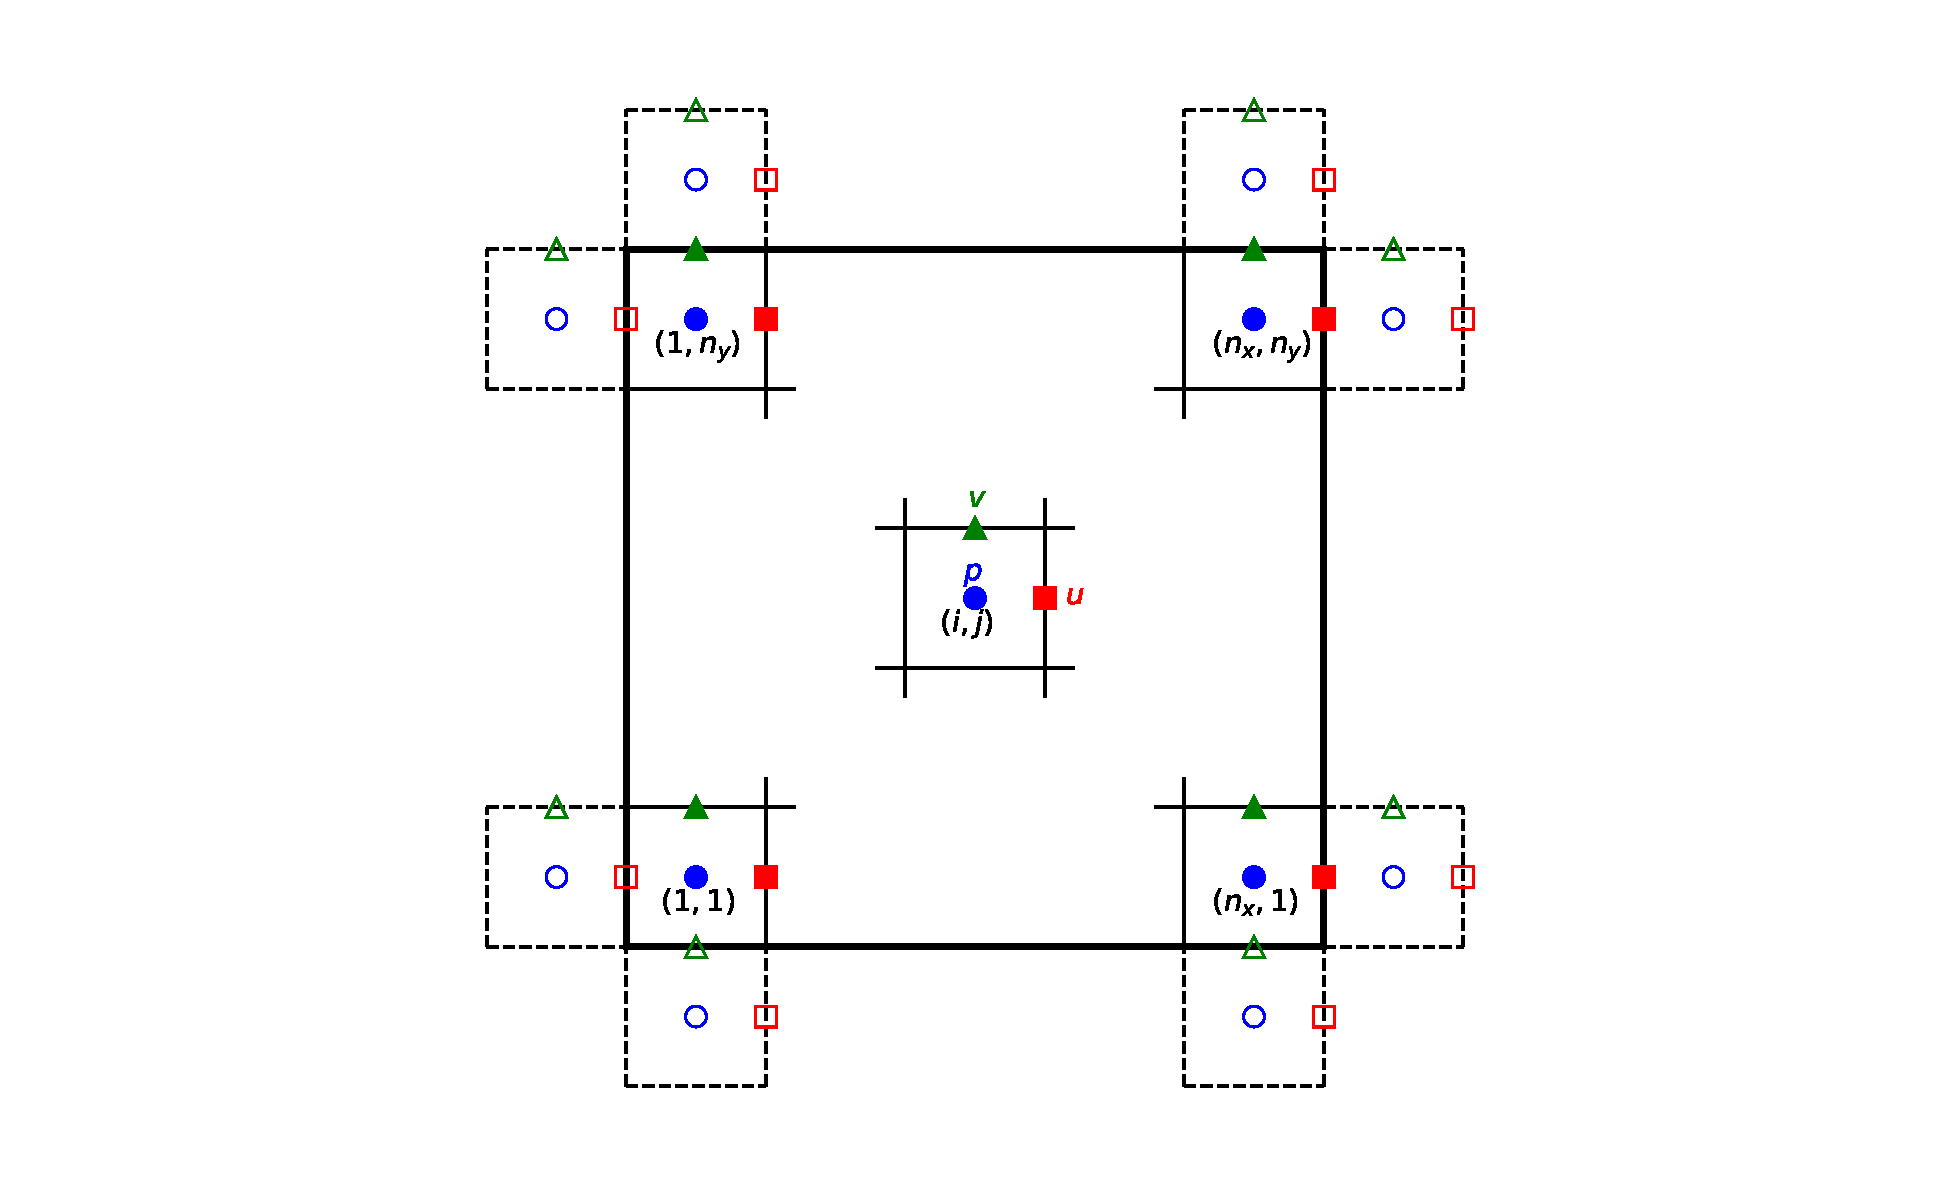
\includegraphics[width=\textwidth]{grid.eps}
    \caption{Sketch of the computational grid. Empty symbols represent ghost nodes.\label{fig:grid}}
\end{figure}


\end{document}